\section{Dataset overview}
\label{sec:dataset}

\begin{figure}
    \centering
    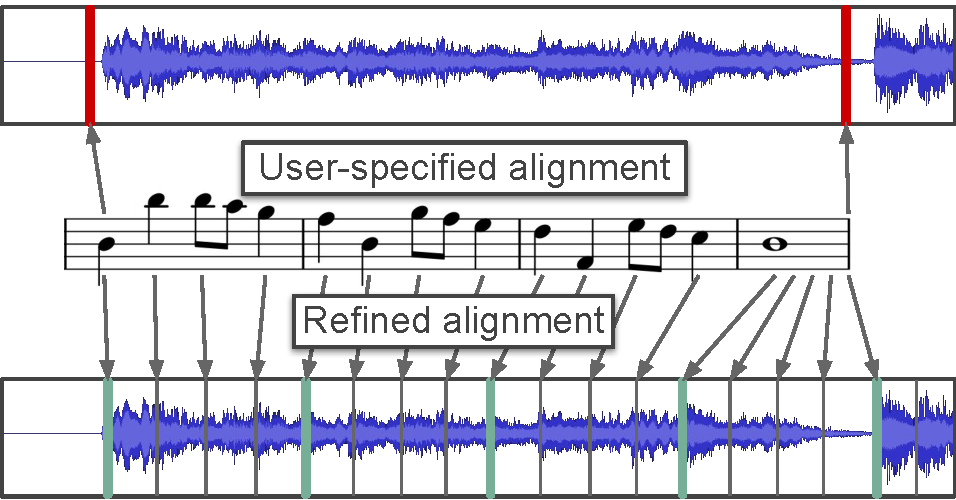
\includegraphics[width=8.1cm]{figs/alignment.pdf}
    \caption{We refine coarse, user-specified alignments from \hooktheory{} by using beat tracking. The first segment beat is mapped to the detected downbeat nearest to the user-specified starting timestamp, and remaining beats are mapped to subsequent detected beats.}
 \label{fig:alignment}
\end{figure}

We collect and release a dataset of crowdsourced melody and chord annotations from \hooktheory{}. 
\hooktheory{} is a platform where users can easily create and share musical analyses of particular recordings hosted on YouTube, with Wikipedia-style editing. 
In lieu of a precise technical definition, these melody annotations constitute a working definition of what musicians perceive as melody. 
The dataset contains annotations for $22$k segments of $13$k unique recordings totaling $50$ hours of labeled audio. 
The audio content covers a wide range of genres---there is a skew towards pop and rock but many other genres are represented including EDM, jazz, and even classical. 
We create an artist-stratified $8$:$1$:$1$ split of the dataset for training, validation, and testing.

\john{Should this paragraph come at the end of the section?}
While data from \hooktheory{} has been used previously for MIR tasks like 
harmonization~\cite{chen2021surprisenet,yeh2021automatic}, 
chord recognition~\cite{jiang2019mirex}, and 
representation learning~\cite{jiang2020transformer}, 
making use of this platform for MIR is currently cumbersome and involves web scraping and reverse engineering a proprietary score format. 
To ease this burden, we release all of the annotations in a simplified JSON format under a Creative Commons license, with links to the audio on YouTube.

\john{This seems a little redundant with \cref{sec:eval}?}
Note that the melody annotations originate from a software tool which uses a ``functional'' annotation format, i.e.,~one which uses scale degrees and roman numerals relative to a key signature instead of absolute notes and chord names. 
The vast majority of transcription work uses absolute labels, hence, we convert these functional labels to absolute ones. 
However, because the annotation tool uses a relative octave format, there is no way to reliably map the melody annotations to the ground truth absolute octave. 
The disregard of absolute octave information on this popular annotation platform implies that a crowd definition of melody does not include this information, reinforcing our earlier argument that it should be ignored for evaluation.

\subsection{Alignment}

\john{Weird to have a single subsection: I commented out a couple sentences below to propose a tighter single-paragraph version that might be moved to top-level \cref{sec:dataset}}
%Included in the release of this dataset is our effort to improve the alignments between the annotations and the audio. \john{Weird topic sentence.}
By default, \hooktheory{} users provide only a coarse alignment, specifying the starting and ending timestamps of the annotated segment. 
%These alignments are overall crude---the starting and ending timestamps are often haphazard, and any tempo fluctuations within a segment will further jeopardize the alignment. \john{Redundant with previous sentence?}
We use the beat and downbeat detection algorithm from \madmom{}~\cite{bock2016joint,bock2016madmom} to refine these alignments. 
Our approach aligns the first beat of the segment to the detected downbeat which is nearest to the user-specified starting timestamp. 
Then, we align the remaining beats to the subsequent detected beats (see~\Cref{fig:alignment} for an example). 
This provides a beat-level alignment for the entire segment, and we use linear interpolation for fractional beat subdivisions. 
In an informal listening test, this produces an improved alignment in around $95\%$ of cases, where the primary failure mode in the remaining $5\%$ occurs when \madmom{} detects the wrong beat as the downbeat. 
We use these refined alignments for training and evaluation, accepting the occasional glitched alignments as noise in the dataset.